\documentclass{article}
\usepackage{graphicx}
\usepackage{float}
\usepackage{subcaption}
\usepackage{amsmath}
\usepackage[colorlinks=true, allcolors=blue]{hyperref}

\bibliographystyle{alpha}

\title{Information Theory \\ \large Problem Set 05 - Stream Codes}
\author{Luís Felipe Ramos Ferreira}
\date{\href{mailto:lframos\_ferreira@outlook.com}{\texttt{lframos\_ferreira@outlook.com}}
}

\begin{document}

\maketitle

\begin{enumerate}
	\item \begin{enumerate}
		      \item Handmade exercise.
		            \begin{figure}[H]
			            \centering
			            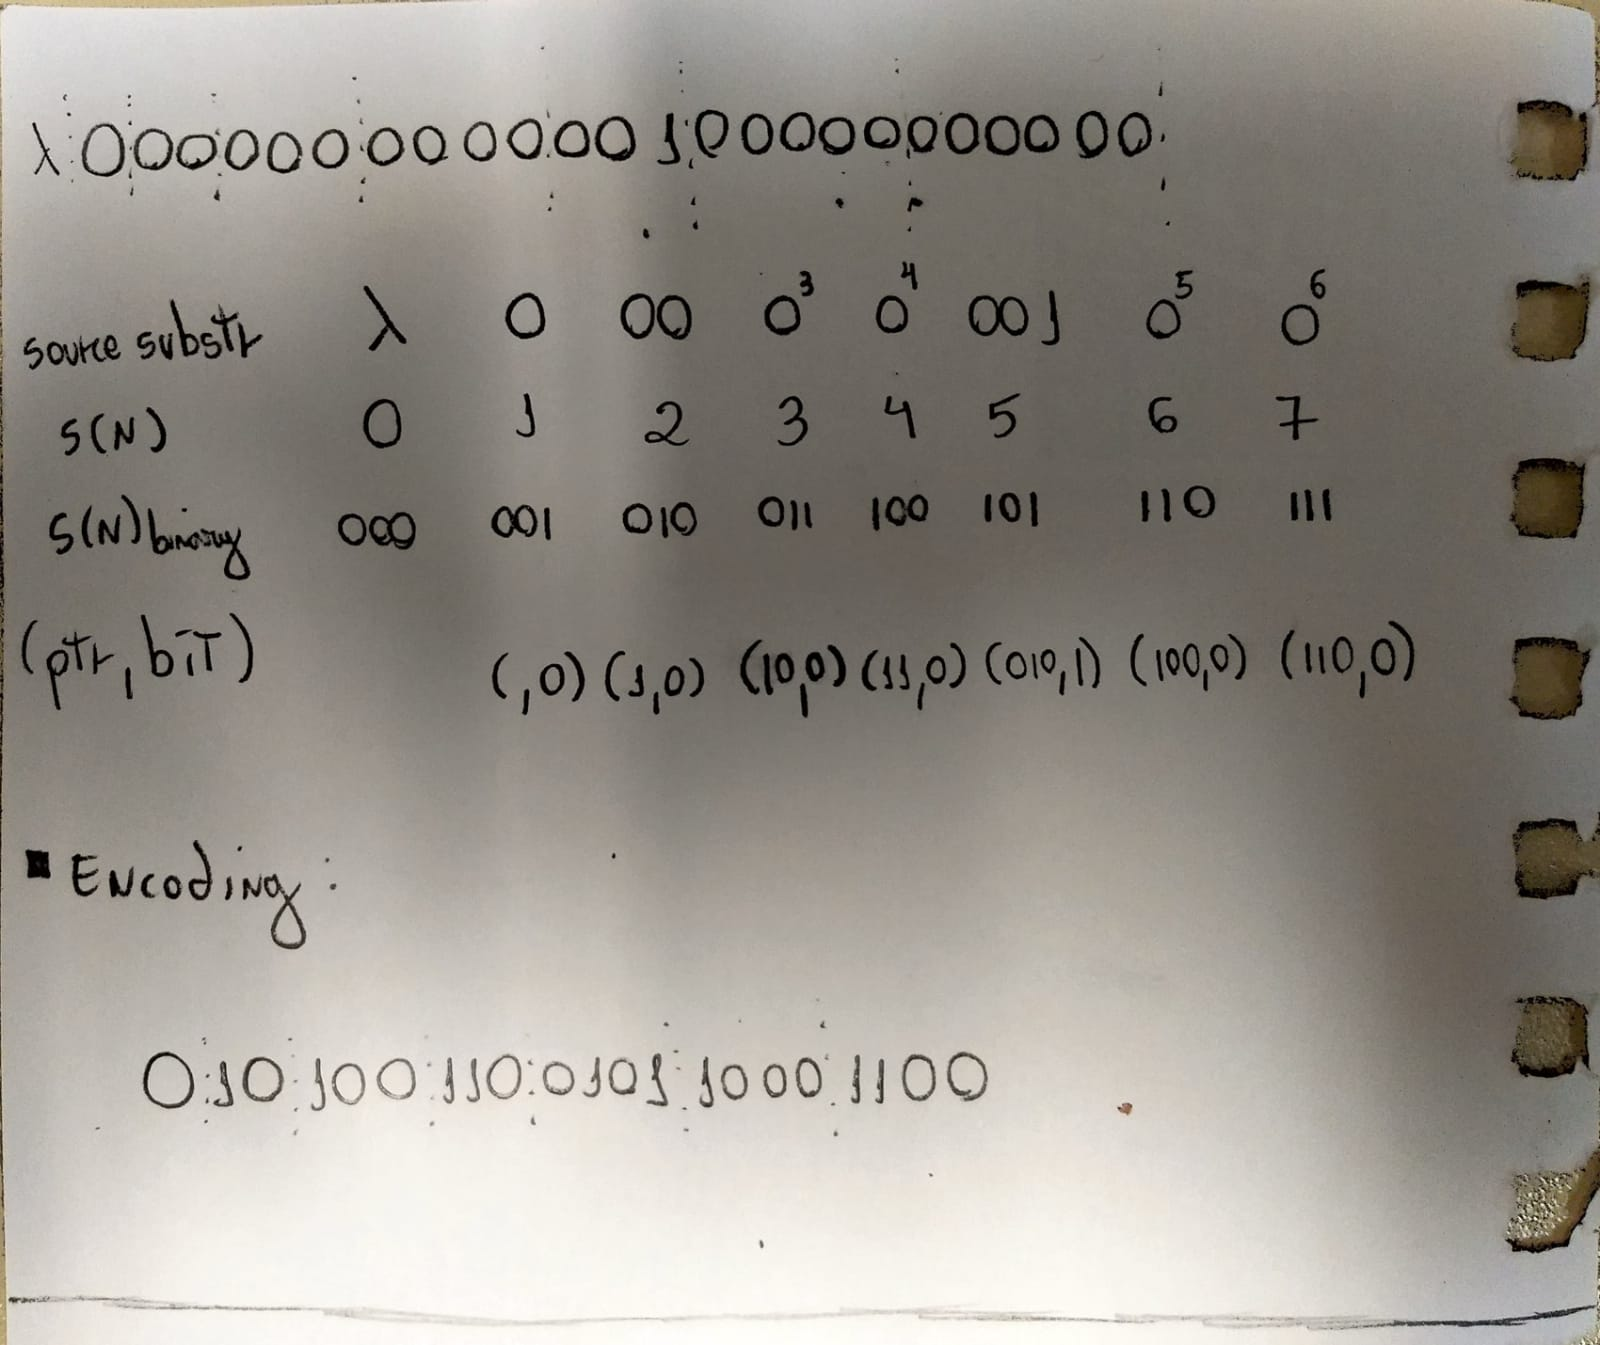
\includegraphics[width=0.8\textwidth]{images/5-1-a.png}
		            \end{figure}

		      \item Handmade exercise.
		            \begin{figure}[H]
			            \centering
			            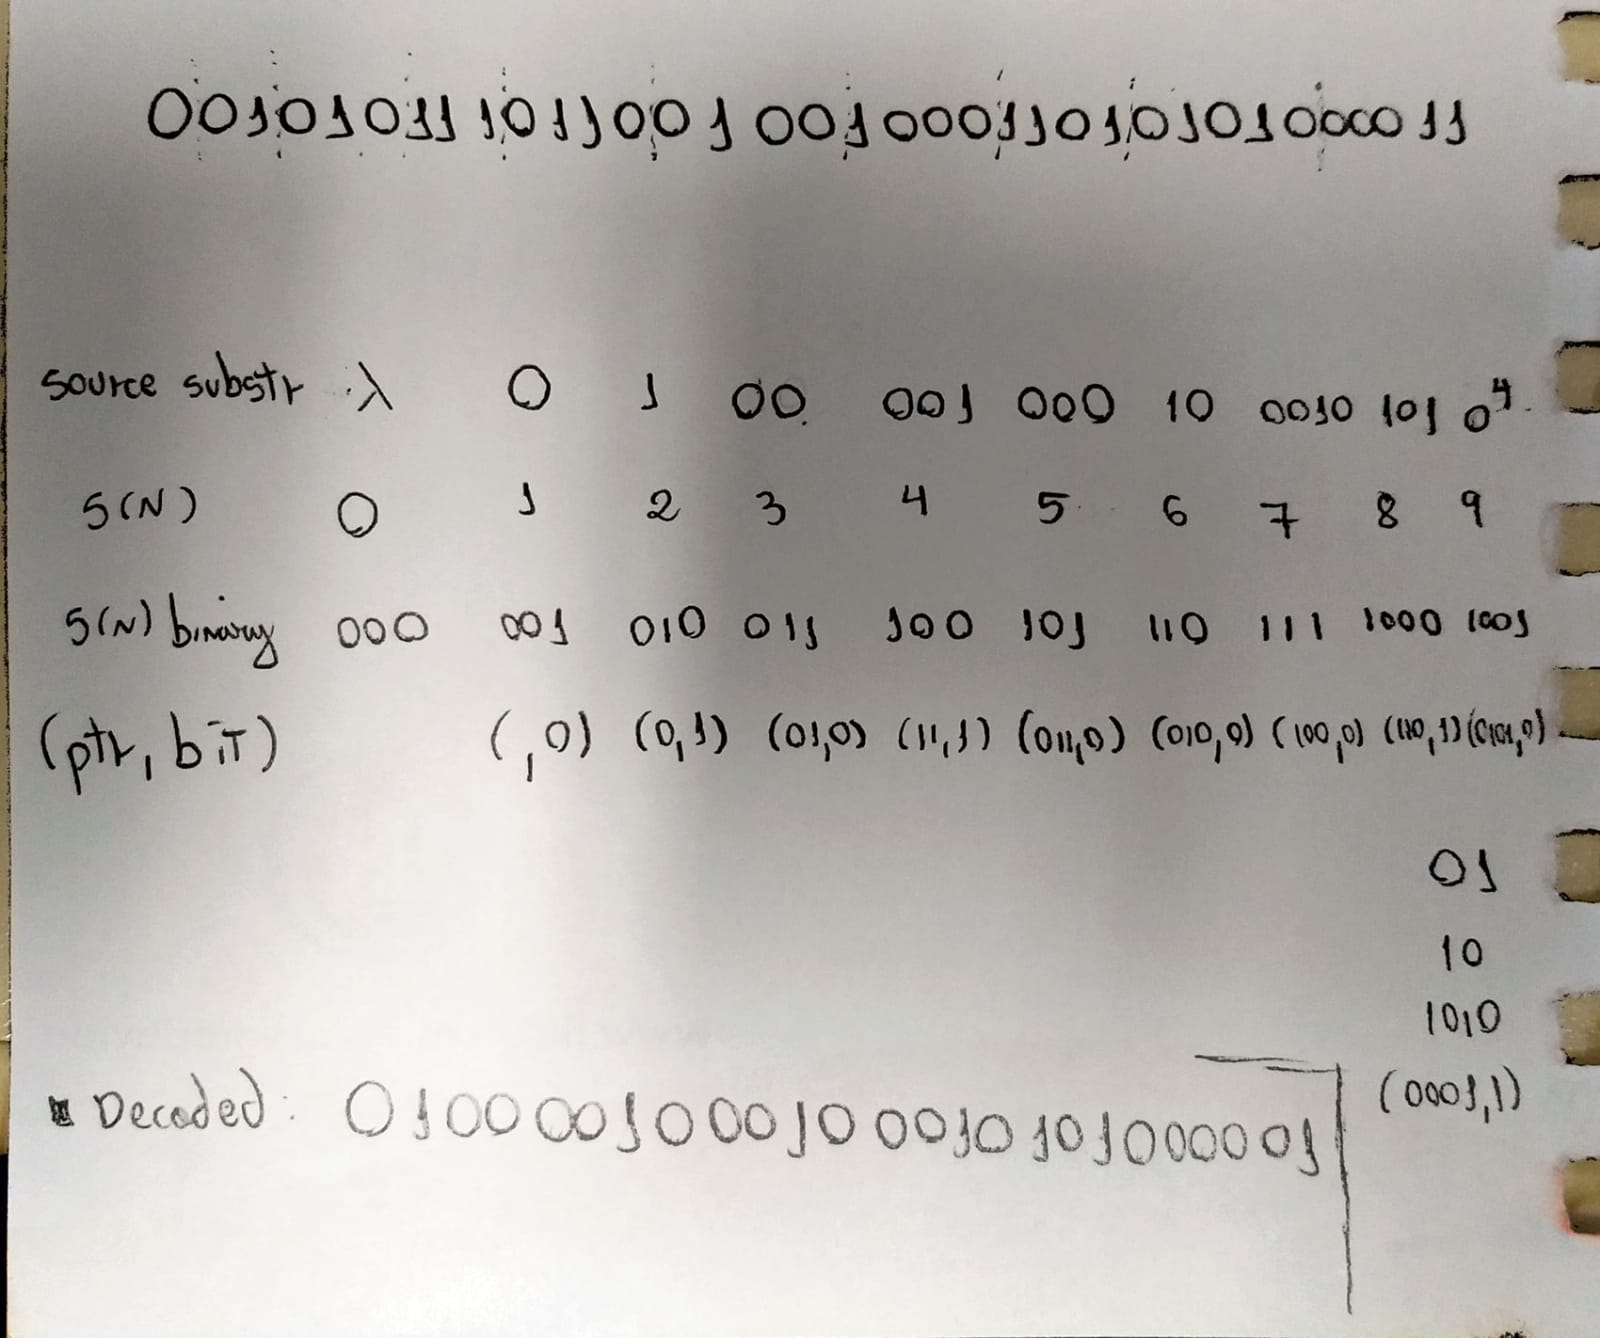
\includegraphics[width=0.8\textwidth]{images/5-1-b.png}
		            \end{figure}
	      \end{enumerate}
	\item \begin{enumerate}
		      \item The three claims from the student are correct. Claims 1 and 2 are true because they basically follow the property stated by the Source Coding Theorem for symbol codes. Claim 3 is true because of a transitive property. Since each symbol in \(X\) is represented in \(Y\) by aproximately \(H(X)\) bits and each symbol in \(Y\) is represente din \(Z\) by aproximately \(H(Y)\), then each symbol in \(X\) is represented in \(Z\) by aproximately \(H(X) H(Y)\) bits.
		      \item b
		      \item c
		      \item d
	      \end{enumerate}
\end{enumerate}
\end{document}
